\documentclass{beamer}
 
\usepackage[utf8]{inputenc}
\usepackage{mathtools}
\usepackage{tikz}
\usetikzlibrary{calc}
\usepackage{graphicx}
\graphicspath{ {./images/} }

\usetheme{CambridgeUS}
\useoutertheme{split}
\setbeamertemplate{title page}[default][colsep=-4bp,rounded=true]

\tikzset{XOR/.style={fill=black!15,draw,minimum size=13pt,circle,append after command={
        [shorten >=\pgflinewidth, shorten <=\pgflinewidth,]
        (\tikzlastnode.north) edge (\tikzlastnode.south)
        (\tikzlastnode.east) edge (\tikzlastnode.west)
        }
    }
}

\tikzstyle{encrypt}=[draw,fill=black!15,rectangle,minimum size=20pt,inner sep=0pt]

 
%Information to be included in the title page:
\title{Block Ciphers}
\author{Rohit Musti}
\institute{CUNY - Hunter College}
\date{\today}
 
\begin{document}
 
\frame{\titlepage}

\begin{frame}
\frametitle{Overview}
\begin{itemize}
    \item \pause We just introduced the concept of stream ciphers and used PRGs to create a basic construction\pause
    \item We also introduced security games \pause
    \item In this lecture, we will build on these ideas and introduce the block cipher a practical cryptography system \pause
\end{itemize}
\end{frame}

\begin{frame}
    \frametitle{One Time Pad Security Game: Chosen Plaintext Attack}
    \begin{tikzpicture}
        % Public parameter:
        
        % Adversary
        \node[draw] (Adversary) at (-3, 2) {\(\mathcal{A}\)}; 
        \draw[thick] (Adversary) -- ++(0, -4); 
        \draw[thick] (Adversary) -- ++(-2, 0);
        \draw[thick] (-3, -2) -- ++(-2, 0);

        % Challenger
        \node[draw] (Challenger) at (3,2) {\(\mathcal{C}\)}; 
        \draw[thick] (Challenger) -- ++(0, -4);
        \draw[thick] (Challenger) -- ++(2, 0);
        \draw[thick] (3, -2) -- ++(2, 0);

        \node[draw=none,fill=none,anchor=east, font=\footnotesize] (choice0) at ($(Adversary) + (0,-.75)$) {\(m_0, m_1 \xleftarrow[]{R} \mathcal{M}\)};
        \draw[->,thick] ($(Adversary)+(0,-1)$) -- ($(Challenger)+(0,-1)$) node [pos=0.5,above,font=\footnotesize] {\(m_0, m_1\)};
        \node[draw=none,fill=none,anchor=west, font=\footnotesize] (bit) at ($(Challenger) + (0,-1.45)$) {\(b \xleftarrow[]{R} \{0, 1\}, k \xleftarrow[]{R} K \)};
        \node[draw=none,fill=none,anchor=west, font=\footnotesize] (bit) at ($(Challenger) + (0,-2.05)$) {\(E(k, m_b) = c\)};
        \draw[->,thick] ($(Challenger)+(0,-2.5)$) -- ($(Adversary)+(0,-2.5)$) node [pos=0.5,above,font=\footnotesize] {\(c \)};
        \draw[->,thick] ($(Adversary)+(2,-2.5)$) -- ($(Adversary)+(2,-1)$) node [pos=0.5,left,font=\footnotesize] {};

        \draw[->,thick] ($(Adversary)+(-1,-4)$) -- ($(Adversary)+(-1,-5)$) node [pos=0.5,left,font=\footnotesize] {\(b\)};
          
          
      \end{tikzpicture}
    
\end{frame}

\begin{frame}
    \frametitle{Pseudo Random Functions (PRFs)}
    \begin{itemize}
        \item \pause \(F: \mathcal{K} \times \mathcal{M} \rightarrow \mathcal{C} \) \pause
        \item  this function must be efficient \pause
        \item  this function is not necessarily one-to-one \pause
        \item  this function is not necessarily invertable \pause
    \end{itemize}
\end{frame}

\begin{frame}
    \frametitle{Pseudo Random Permutation (PRPs)}
    \begin{itemize}
        \item \pause \(P: \mathcal{K} \times \mathcal{X} \rightarrow \mathcal{X} \) \pause
        \item  this function must be efficient \pause
        \item  this function is one-to-one \pause
        \item  there exists an efficient algorithm for inverting this \pause
    \end{itemize}
\end{frame}

\begin{frame}
    \frametitle{Security of PRPs and PRFs}
    \begin{itemize}
        \item \pause A PRF \(F: \mathcal{K} \times \mathcal{M} \rightarrow \mathcal{C} \) is secure  if \(F(k, \cdot)\) is indistinguishable from a random function \(f \xleftarrow[]{R} (\mathcal{M} \rightarrow \mathcal{C})\) \pause
        \item a PRP  \( P: \mathcal{K} \times \mathcal{X} \rightarrow \mathcal{X} \) is secure if \(P(k, \cdot)\) is indistinguishable from a random permutation \(p \xleftarrow[]{R} (\mathcal{X} \rightarrow \mathcal{X})\)
    \end{itemize}
\end{frame}


\begin{frame}
    \frametitle{PRF Security Game: Chosen Plaintext Attack}
    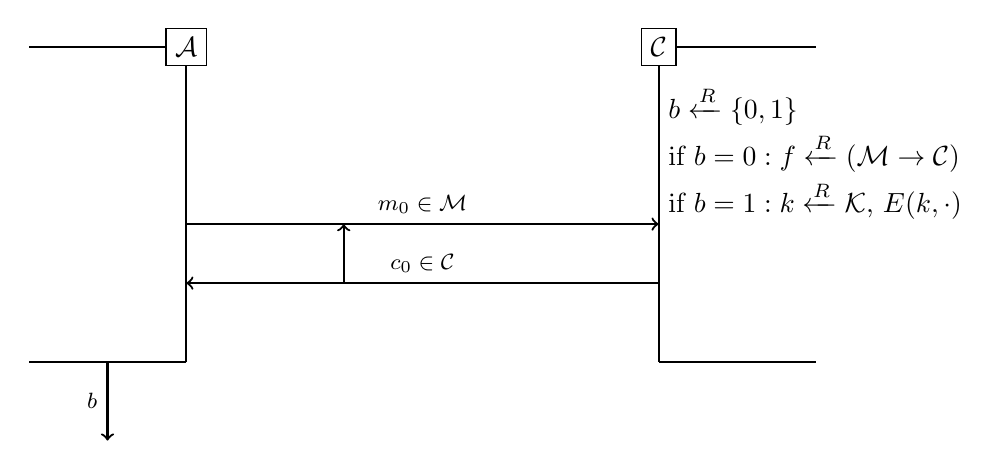
\begin{tikzpicture}
        % Public parameter:
        
        % Adversary
        \pause
        \node[draw] (Adversary) at (-3, 2) {\(\mathcal{A}\)}; 
        \draw[thick] (Adversary) -- ++(0, -4); 
        \draw[thick] (Adversary) -- ++(-2, 0);
        \draw[thick] (-3, -2) -- ++(-2, 0);
        \pause

        % Challenger
        \node[draw] (Challenger) at (3,2) {\(\mathcal{C}\)}; 
        \draw[thick] (Challenger) -- ++(0, -4);
        \draw[thick] (Challenger) -- ++(2, 0);
        \draw[thick] (3, -2) -- ++(2, 0);
        \pause

        \node[draw=none,fill=none,anchor=west] (bit) at ($(Challenger) + (0,-.75)$) {\(b \xleftarrow[]{R} \{0, 1\} \)};
        \pause
        \node[draw=none,fill=none,anchor=west] (choice0) at ($(Challenger) + (0,-1.35)$) {if \(b = 0: f \xleftarrow[]{R}(\mathcal{M} \rightarrow \mathcal{C}) \)};
        \pause
        \node[draw=none,fill=none,anchor=west] (choice1) at ($(Challenger) + (0,-1.95)$) {if \(b = 1: k \xleftarrow[]{R} \mathcal{K} \), \(E(k, \cdot )\)};
        \pause
        \draw[->,thick] ($(Adversary)+(0,-2.25)$) -- ($(Challenger)+(0,-2.25)$) node [pos=0.5,above,font=\footnotesize] {\(m_0 \in \mathcal{M} \)};
        \pause
        \draw[->,thick] ($(Challenger)+(0,-3)$) -- ($(Adversary)+(0,-3)$) node [pos=0.5,above,font=\footnotesize] {\(c_0 \in \mathcal{C} \)};
        \pause
        \draw[->,thick] ($(Adversary)+(2,-3)$) -- ($(Adversary)+(2,-2.25)$) node [pos=0.5,left,font=\footnotesize] {};
        \pause

        \draw[->,thick] ($(Adversary)+(-1,-4)$) -- ($(Adversary)+(-1,-5)$) node [pos=0.5,left,font=\footnotesize] {\(b\)};
          
          
      \end{tikzpicture}
    
\end{frame}

\begin{frame}
    \frametitle{PRP Security Game: Chosen Plaintext Attack}
    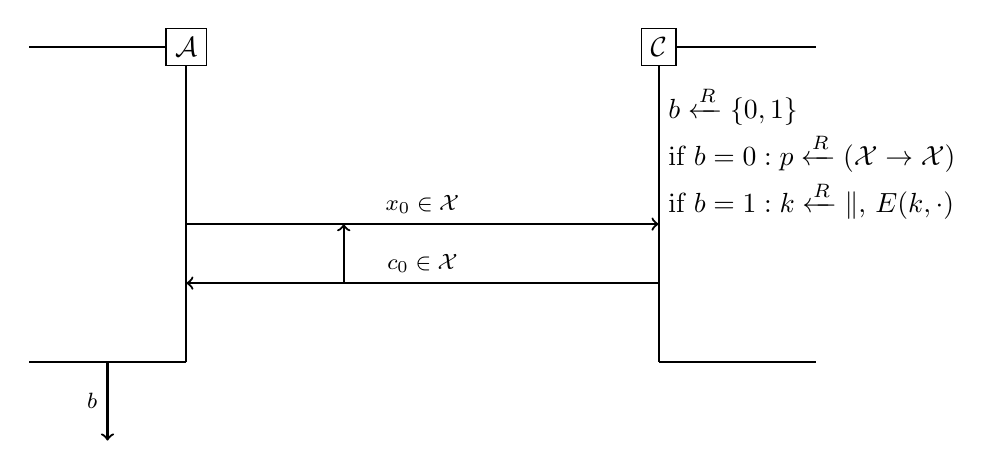
\begin{tikzpicture}
        % Public parameter:
        
        % Adversary
        \pause
        \node[draw] (Adversary) at (-3,2) {\(\mathcal{A}\)}; 
        \draw[thick] (Adversary) -- ++(0, -4); 
        \draw[thick] (Adversary) -- ++(-2, 0);
        \draw[thick] (Adversary) -- ++(-1, 0);
        \draw[thick] (-3, -2) -- ++(-2, 0);
        \pause

        % Challenger
        \node[draw] (Challenger) at (3,2) {\(\mathcal{C}\)}; 
        \draw[thick] (Challenger) -- ++(0, -4);
        \draw[thick] (Challenger) -- ++(2, 0);
        \draw[thick] (3, -2) -- ++(2, 0);
        \pause

        \node[draw=none,fill=none,anchor=west] (bit) at ($(Challenger) + (0,-.75)$) {\(b \xleftarrow[]{R} \{0, 1\} \)};
        \pause
        \node[draw=none,fill=none,anchor=west] (choice0) at ($(Challenger) + (0,-1.35)$) {if \(b = 0: p \xleftarrow[]{R}(\mathcal{X} \rightarrow \mathcal{X}) \)};
        \pause
        \node[draw=none,fill=none,anchor=west] (choice1) at ($(Challenger) + (0,-1.95)$) {if \(b = 1: k \xleftarrow[]{R} \mathcal{k} \), \(E(k, \cdot )\)};
        \pause
        \draw[->,thick] ($(Adversary)+(0,-2.25)$) -- ($(Challenger)+(0,-2.25)$) node [pos=0.5,above,font=\footnotesize] {\(x_0 \in \mathcal{X}\)};
        \pause
        \draw[->,thick] ($(Challenger)+(0,-3)$) -- ($(Adversary)+(0,-3)$) node [pos=0.5,above,font=\footnotesize] {\(c_0 \in \mathcal{X} \)};
        \pause
        \draw[->,thick] ($(Adversary)+(2,-3)$) -- ($(Adversary)+(2,-2.25)$) node [pos=0.5,left,font=\footnotesize] {};
        \pause

        \draw[->,thick] ($(Adversary)+(-1,-4)$) -- ($(Adversary)+(-1,-5)$) node [pos=0.5,left,font=\footnotesize] {\(b\)};
      \end{tikzpicture}
    
\end{frame}

\begin{frame}
\frametitle{Security Lemma}
\begin{itemize}
    \item a secure PRP is equivalent to a secure PRF
\end{itemize}
\end{frame}

\begin{frame}
\frametitle{Block Ciphers}
\begin{itemize}
    \item \pause block ciphers can be thought of as PRPs \pause
    \item block ciphers are deterministic ciphers \( \mathcal{E} = (E, D) \)\pause
    \item its message space and ciphertext space are the same: \( \mathcal{M} = \mathcal{C} \) \pause
    \item Shares the correctness requirement with Shannon Ciphers \( D(k, E(k, m)) = m \)
\end{itemize}
\end{frame}

\begin{frame}
    \frametitle{History: Electronic Code Book}
    \begin{itemize}
        \item \pause Developed by IBM in the 1970s, became an official Federal Information Processing Standard in 1977 \pause
        \item Released with 4 other ciphers, all of which were more secure, but not totally secure on their own \pause
        \item Name derives the code books used during the Civil War \pause
    \end{itemize}

\end{frame}

\begin{frame}
    \frametitle{How it Works: Electronic Code Book}

	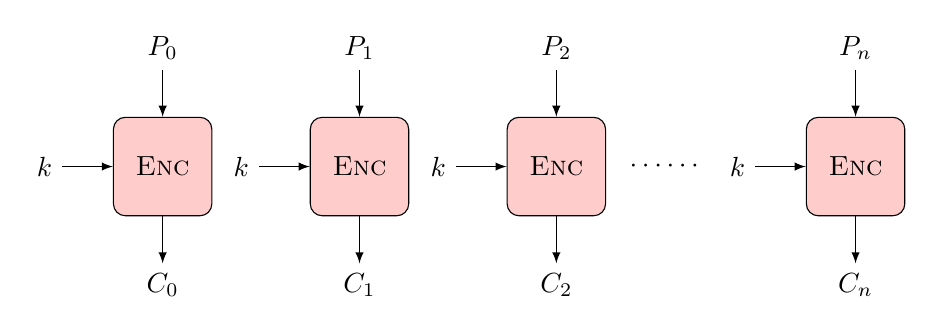
\begin{tikzpicture}
    
        \foreach \x in {0, 1, 2} {
            \node (f\x) at ($\x*(2.5cm,0)$) [minimum size=1.25cm,rounded corners=1ex,fill=red!20,draw] {{\sc Enc}};
            \node (m\x) [above of=f\x, node distance=1.5cm] {$P_\x$};
            \node (k\x) [left of=f\x, node distance=1.5cm] {$k$};
            \node (c\x) [below of=f\x, node distance=1.5cm] {$C_\x$};
            \draw[-latex] (m\x) -- (f\x);
            \draw[-latex] (k\x) -- (f\x);
            \draw[-latex] (f\x) -- (c\x);
            \pause
        }

        \begin{scope}
            \node at (6.4,0) {$\cdots\cdots$};
        \end{scope}

        \begin{scope}
            \node (f) at (8.8cm,0) [minimum size=1.25cm,rounded corners=1ex,fill=red!20,draw] {{\sc Enc}};
            \node (m) [above of=f, node distance=1.5cm] {$P_n$};
            \node (k) [left of=f, node distance=1.5cm] {$k$};
            \node (c) [below of=f, node distance=1.5cm] {$C_n$};
            \draw[-latex] (m) -- (f);
            \draw[-latex] (k) -- (f);
            \draw[-latex] (f) -- (c);
        \end{scope}
        
    \end{tikzpicture}
    \vfill
    \textit{Image Credit: }Diana Maimut
\end{frame}

\begin{frame}
    \frametitle{Security Weakness: Electronic Code Book}
    \begin{itemize}
        \item \pause since the encryption function is a PRP, it is deterministic and one-to-one \pause
        \item therefore, it \(m_1 = m_2\), then it follows that \(c_1 = c_2\) \pause
        \item this doesn't achieve chosen plaintext attack security\pause
    \end{itemize}
        Future HW: describe an attack to break CPA given ECB
\end{frame}

\begin{frame}
    \frametitle{Image Encryption using ECB}
    \begin{figure}
        \begin{center}
            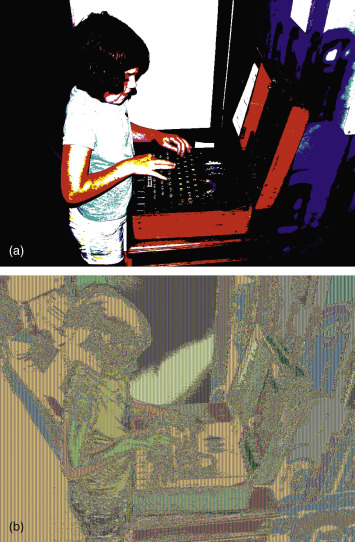
\includegraphics[scale=0.6]{image_ecb.jpg}
        \end{center}
    \end{figure}
    \textit{Image Credit: }\href{https://www.sciencedirect.com/topics/computer-science/electronic-code-book}(the NSA)
\end{frame}

\begin{frame}
    \frametitle{Cipher Block Chaining: CBC (not quite cryptocurrencies)}
    \begin{figure}
        \begin{center}
            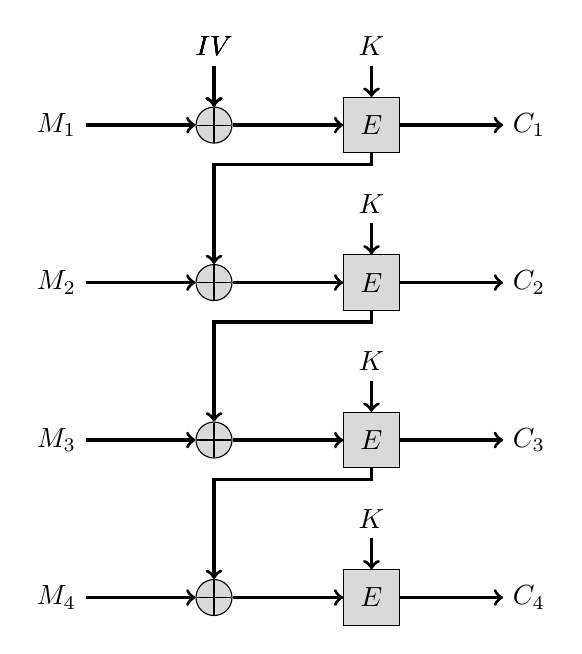
\begin{tikzpicture}
                \pause 

                \newcommand{\n}{4}
                \foreach \nr in {1, ..., \n}{
                    \node (M\nr)            at (0,{(\n-\nr)*2}) {$M_\nr$};
                    \node (x\nr)[XOR]       at (2,{(\n-\nr)*2}) {};
                    \node (E\nr)[encrypt]   at (4,{(\n-\nr)*2}) {$E$};
                    \node (C\nr)            at (6,{(\n-\nr)*2}) {$C_\nr$};
    
                    \node (K\nr)            at (4,{(\n-\nr)*2+1}) {$K$};
    
                    \draw[->,very thick] (M\nr) -- (x\nr);
                    \draw[->,very thick] (x\nr) -- (E\nr);
                    \draw[->,very thick] (E\nr) -- (C\nr);
    
                    \draw[->,very thick] (K\nr) -- (E\nr);


                    \node (IV) at (2,{\n*2-1}) {$IV$};
                    \draw[->, very thick] (IV) -- (x1);
                    \pause
                }
    
                \foreach \nr in {2, ..., \n}{
                    \pgfmathtruncatemacro{\tmp}{\nr-1}
                    \draw[->,very thick] (E\tmp) -- (4, {(\n-\tmp)*2-0.5}) -- (2, {(\n-\nr)*2+1.5}) -- (x\nr);
                }
    
    
            \end{tikzpicture}
        \end{center}
    \end{figure}
    \textit{Image Credit: }\href{https://github.com/MartinThoma/LaTeX-examples/blob/master/tikz/CBC-Mode-Encryption/CBC-Mode-Encryption.tex}(Martin Thoma)
\end{frame}

\begin{frame}
    \frametitle{CBC: Picking a good IV}
    \begin{itemize}
        \item \pause If you are developing a single use system, you do not even need an IV \pause
        \item You can use a unique IV (i.e. counter mode) but then you have to sample a new IV each round, but you don't need to send the IV with the cipher text \pause
        \item It is best to use a random IV every message and send it with the cipher text 
    \end{itemize}
\end{frame}

\begin{frame}
    \frametitle{Advanced Encryption System (AES)}
    \begin{itemize}
        \item \pause Developed by two belgian cryptographers,  Joan Daemen and Vincent Rijmen \pause
        \item Adopted by US government, supersedes DES (the one that contained EBC), in 2002 \pause
        \item First and only publicly accessible cypher approved by NSA 
    \end{itemize}
    
\end{frame}

\begin{frame}
    \frametitle{Advanced Encryption System (AES)}
    \begin{enumerate}
        \item \pause Derive round keys using key scheduler from cipher key \pause
        \item Expand the current key into the \textit{round} key \pause
        \item Complete encryption rounds \pause
        \begin{enumerate}
            \item Non linear byte substitution according to look up table\pause
            \item Shift rows: last 3 rows are cyclically shifted\pause
            \item Mix Columns: combine four bytes in each column according to a linear mixing operation\pause
            \item XOR with round key
        \end{enumerate}
        \item Final encryption round\pause
        \begin{enumerate}
            \item Non linear byte substitution according to look up table\pause
            \item Shift rows: last 3 rows are cyclically shifted\pause
            \item XOR with round key\pause
        \end{enumerate}
    \end{enumerate}
\end{frame}

\end{document}
